\documentclass[12pt]{article}
\RequirePackage[colorlinks,citecolor=blue,urlcolor=blue]{hyperref}
\usepackage[utf8]{inputenc}
\usepackage{csquotes}
\usepackage[authordate, backend=biber, maxcitenames=2,ibidtracker=false]{biblatex-chicago}
\addbibresource{refs.bib}
\usepackage{amsmath, amssymb}
\usepackage{graphicx,bm}
\usepackage{color}
\usepackage{subcaption}
\usepackage{rotating}
\usepackage{eurosym}
\usepackage{colonequals}
\usepackage{bbm}
\usepackage{lscape}
\usepackage{float}
\usepackage{amsfonts,amsthm}
\usepackage[english]{babel}
\usepackage[colorinlistoftodos]{todonotes}
\usepackage{enumitem}
\usepackage{listings}
\usepackage{verbatim}
\usepackage{mathtools, calc}  
\usepackage{neuralnetwork}
\usepackage{tikz}
\usepackage[export]{adjustbox}
\setlength {\marginparwidth }{2cm} 
\begin{document}

%----------------------------------------------------------------------------------------
%	TITLE SECTION
%----------------------------------------------------------------------------------------
\begin{titlepage}

  \newcommand{\HRule}{\rule{\linewidth}{0.5mm}}
  \center

  \textsc{\LARGE McMaster University}\\[1.5cm]
  \textsc{\Large STATS 771}\\[0.5cm]
  \textsc{\large Statistical Research Project}\\[0.5cm]

  \HRule \\[0.4cm]
  { \huge \bfseries Feature Extraction and Selection Techniques for Handling High-Dimensional Data in NLP}\\[0.4cm]
  \HRule \\[1.5cm]

  \begin{minipage}{0.4\textwidth}
    \begin{flushleft} \large
      \emph{Author:}\\
      Tolu \textsc{Olusooto}
      \textit{(1235801)}\\
    \end{flushleft}
  \end{minipage}
  ~
  \begin{minipage}{0.4\textwidth}
    \begin{flushright} \large
      \emph{Professor:} \\
      Dr. Angelo J. \textsc{Canty}\\
      \textit{} \\
    \end{flushright}
  \end{minipage}\\[2cm]

  {\large \today}\\[2cm]


  \vfill
  \newpage

  %----------------------------------------------------------------------------------------
  %	ABSTRACT SECTION
  %----------------------------------------------------------------------------------------
  \begin{abstract}
    This paper examines the curse of dimensionality in Natural Language Processing (NLP) and its impact on model overfitting. The focus of the paper is to compare 3 dimension reduction techniques (DRTs) - Latent Semantic Analysis (LSA), Linear Discriminant Analysis (LDA), and Auto-Encoder (AE) - used in text classification tasks. The paper is divided into four main sections - Data, Literature Review, Experiment, and Conclusion. The Data section analyzes the dataset used and describes the preprocessing steps. The Literature Review section showcases prior applications and observations of the DRTs investigated in this paper. The Experiment section outlines the methodology used to compare the DRTs, and the results of the experiment are presented. The Conclusion section highlights the key findings of the paper, with the TF-IDF method being the most efficient and effective reduction technique in terms of classification accuracy and computational time. The Conclusion section highlights the key findings of the paper. The TF-IDF method is found to be the most efficient and effective reduction technique in terms of classification accuracy and computational time.
  \end{abstract}

\end{titlepage}

%----------------------------------------------------------------------------------------
%	INTRODUCTION SECTION
%----------------------------------------------------------------------------------------
\section{Introduction}
\hspace{\parindent} Natural Language Processing (NLP) is defined as a set of techniques used by computers to process and/or synthesize human languages \parencite{eisenstein_2019}. In recent years, NLP has become more integrated into our daily lives thanks to the advancements in technology and machine learning (ML). From tools such as Google Translate, email classification, and most recently ChatGPT, NLP-based tasks have made it easier for people to communicate and share information. NLP is an interdisciplinary topic drawing concepts from subjects such as computational linguistics, statistics, and artificial intelligence \parencite{eisenstein_2019}.

Though there are many societal benefits gained from the use of NLP, the computational and statistical challenges from processing such high dimensional data (HDD), a dataset where the number of parameters is large relative to the data sample or larger than data sample, can be quite a strain \parencite{buehlmann_peter_van_de_geer_2013}. These limitations can lead to a reduction in processing speed and classification accuracy \parencite{ayesha_hanif_talib_2020}. When processing HDD in ML, a known statistical problem tends to occur: curse of dimensionality. Curse of dimensionality is for every small increase in dimension or parameter in the dataset, an exponentially larger increase in data sample is needed for an accurate prediction or classification to be made by the model \parencite{ayesha_hanif_talib_2020}. A symptom of curse of dimensionality is model overfitting. That is increasing the dimensions of the data improves the model performance; however, past a certain dimensionality, this will have the opposite effect \parencite{ayesha_hanif_talib_2020}. The effects of overfitting a model are a noticeable decline in performance from the training to testing set. With regards to NLP data such as text, also known as corpus, another common symptom of curse of dimensionality is data sparsity \parencite{another_look}. Data sparsity is when the training set does not contain enough features or words to accurately classify text samples outside the training set, leading the model to overfit \parencite{another_look}.

To address the curse of dimensionality, there is a class of ML algorithms known as dimensionality reduction techniques (DRT) that can be used. These techniques fall into one of two categories: feature selection and feature extraction \parencite{ayesha_hanif_talib_2020}. Feature selection involves subsetting the most relevant features in the dataset relative to the given task, while feature extraction transforms the data to a lower dimension while retaining the most important information \parencite{ayesha_hanif_talib_2020}.

\subsection{Motivation}
\hspace{\parindent} With the increasing amount of data being generated for NLP models such as BERT and ChatGPT to process, the issue of model overfitting becomes a significant concern. While computational advancements such as GPUs and cloud computing have facilitated the development and training of larger models, statistical advancements like DRT are employed to mitigate overfitting issues associated with these models. This paper aims to compare the most common DRTs used in text classification today. To keep the paper concise, only 3 DRTs were examined in detail. These include one supervised, one unsupervised and one semi-supervised method. Latent Semantic Analysis (LSA) was the unsupervised method used, while Linear Discriminant Analysis (LDA) was the supervised method used. Finally, Auto-Encoder (AE) was the semi-supervised method chosen.

The paper is divided into four main sections, namely Data, Literature Review, Experiment, and Conclusion. In the Data section, the dataset used is analyzed and the preprocessing steps are detailed. The Literature Review section showcases some prior applications and observations of the 3 DRTs investigated in this paper by other studies. Additionally, this section provides a theoretical derivation of each DRT. The Experiment sections describes the methodology used to compare the DRTs and the results of the experiment is presented. Lastly, the Conclusion section summarizes the key findings of the paper.

\section{Data}
\hspace{\parindent} The data used in this paper is called 'BBC News Archive' \parencite{greene06icml}. The dataset contains 2,225 news articles published by BBC News from 2004-2005 \parencite{greene06icml}. These articles are classified into one of five topics: (Business, Entertainment, Politics, Sport, Tech). The data was made available by Derek Greene and P\'{a}draig Cunningham; who used it in their 2006 paper 'Practical Solutions to the Problem of Diagonal Dominance in Kernel Document Clustering'. Both the processed and raw data were made available, and for the purpose of this paper the processed data will be used. Processed data contains 4 columns: the article title, filename, news category and content of the article \parencite{greene06icml}.

\subsection{Data Preprocessing}
\hspace{\parindent} All the data wrangling was done using the \texttt{python} library \texttt{pandas} \parencite{mckinney2010data}. During the cleaning stage, 98 duplicate articles were removed. The title and content of each article were merged into a single column named "text," forming a comprehensive corpus. Additionally, a encoded representation of the categories was generated, while the filename, content, and title columns were discarded.

After processing the data, exploratory data analysis (EDA) was performed, revealing an imbalance in the data with the majority of the articles being either sports or business-related. The tech articles represented the smallest share. However, the overall difference between the categories is relatively small, with the most significant difference from the expected ratio being 4\%. The imbalance in data will not be addressed as it is the reality of real-world datasets and the level of imbalance is minimal. The EDA also revealed that some high-frequencies words were common amongst all 5 categories, which did not assist in distinguishing them from one another. The words \texttt{"said"} and \texttt{"will"} were the most common words in the dataset. Given that the dataset comprises news articles, it is reasonable to see the heavy representation of these verbs in the dataset.

\begin{figure}[H]
  \centering
  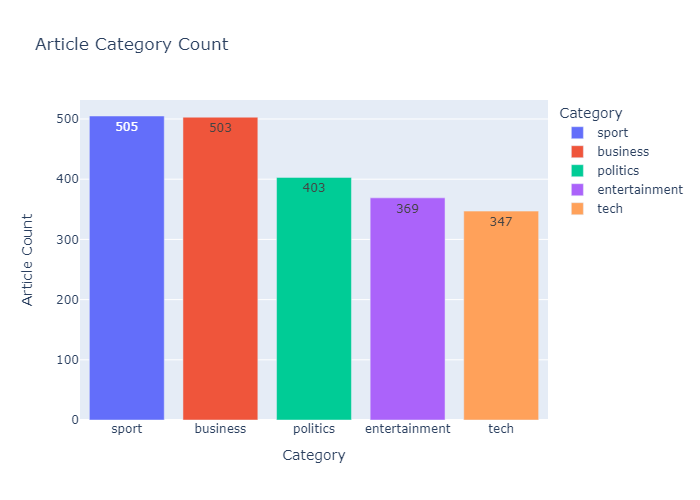
\includegraphics[scale=0.55]{plots/barplot.png}
  \caption{The article count for each of the 5 categories.}
\end{figure}

\begin{table}[H]
  \centering
  \resizebox{.60\textwidth}{!}{%
    \begin{tabular}{|c|c|c|c|}
      \hline
      Category      & Expected Ratio & Actual Ratio & Difference \\ \hline
      sport         & 20\%           & 23.74\%      & 3.74\%     \\
      business      & 20\%           & 23.65\%      & 3.65\%     \\
      politics      & 20\%           & 18.95\%      & 1.05\%     \\
      entertainment & 20\%           & 17.35\%      & 2.65\%     \\
      tech          & 20\%           & 16.31\%      & 3.69\%
      \\ \hline
    \end{tabular}%
  }
  \caption{The deviation from the expected distribution for each of the 5 categories.}
\end{table}

The processed data was further cleaned by removing numbers and symbols and converting all the words to lowercase in each text. Furthermore, stopwords were dropped from the text. Stopwords are words in text that add little to no contribution to the overall message or topic of the text \parencite{eisenstein_2019_2}. Some examples of stopwords are \texttt{"the," "a," "said," "will,"} and \texttt{"for."} Stopwords removal is good practice in NLP since they offer negligible discriminatory power when assigning a text to one of the five categories. Their inclusion may introduce noise to the model, which could ultimately decrease its accuracy \parencite{manning_raghavan_schütze_2009}. The removal of stopwords is a feature selection technique as it reduces the number of words that the model has to process. A comprehensive list of stopwords was referenced during the stopwords removal process, the list is a combination of stopwords from the \texttt{nltk} library and the \texttt{stopwordsiso} library \parencite{bird2009natural}; \parencite{stopwordsiso}.

Continuing with NLP best practices, the dataset was normalized through lemmatization after removing stopwords \parencite{bird2009natural_lem}. Lemmatization is the reduction of a word to its root form or lemma, for example, converting \texttt{"running"} or \texttt{"ran"} to \texttt{"run"} \parencite{manning_raghavan_schütze_2009_stem_lem}. This process takes into account a word's morphology and matches the resulting lemma against a vocabulary set, ensuring it is a valid word \parencite{manning_raghavan_schütze_2009_stem_lem}. The \texttt{nltk} library's \texttt{WordNetLemmatizer} module was used to lemmatize the dataset \parencite{bird2009natural}. However, further analysis of the corpus found the module did not accurately interpret certain words, specifically acronyms. Words such as \texttt{"US"}, short for United States, or \texttt{"OS"}, short for operating systems, were treated as plurals of the letters \texttt{"U"} and \texttt{"O"}, respectively. To solve this issue, a conditional statement was added to exclude these acronyms from lemmatization. After applying the aforementioned processes, the dataset went from 65,553 potential features to 24,134, which is more than a 63\% reduction in potential features.

\begin{figure}[H]
  \centering
  \begin{tabular}{cc}
    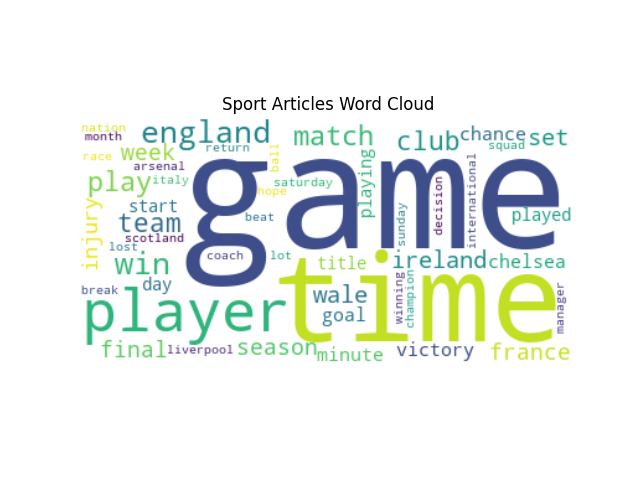
\includegraphics[scale=0.50]{plots/sport_wordcloud.png}    &
    
\includegraphics[scale=0.50]{plots/business_wordcloud.png}      \\
    
\includegraphics[scale=0.50]{plots/politics_wordcloud.png} &
    
\includegraphics[scale=0.50]{plots/entertainment_wordcloud.png} \\
    
\includegraphics[scale=0.50]{plots/tech_wordcloud.png}          \\
  \end{tabular}
  \caption{The wordclouds are created from the cleaned dataset, showing the most common words within each of the 5 categories.}
\end{figure}

The wordclouds shown above were generated using the \texttt{wordcloud} library in Python \parencite{oesper2011wordcloud}. Based on these wordclouds, it is apparent that certain highly distinctive topical words appear quite frequently within each category. However, it is worth noting that generic words such as \texttt{"people"} and \texttt{"time"} are also amongst some of the most common words within each category.

The bag-of-words (BoW) module from Python's \texttt{sklearn} library was used to transform the dataset into vectors \parencite{pedregosa2011scikit}. The BoW method represents each unique word as a column, and each article in the dataset as a row \parencite{manning_raghavan_schütze_2009_tf}. A frequency count is given to each word depending on how often it appears within an article, regardless of the word's context \parencite{manning_raghavan_schütze_2009_tf}. The transformed dataset is now a document-term matrix with 2,127 rows representing the articles and 24,134 columns representing the count of unique words. Most of the values in this matrix will be 0, making it a sparse matrix.

The Term Frequency-Inverse Document Frequency (TF-IDF) formula was applied to the BoW vectors, resulting in a numerical representation of the relevance of each word within a particular article, with respect to the other articles \parencite{manning_raghavan_schütze_2009_tf}. TF-IDF is the product of the term frequency (TF) and inverse document frequency (IDF) \parencite{manning_raghavan_schütze_2009_tf}. TF is the number of times a word appears within an article, while IDF measures the significance of that word in determining the category of the article \parencite{manning_raghavan_schütze_2009_tf}. The TF-IDF formula is as follows \parencite{manning_raghavan_schütze_2009_tf}:

\begin{equation}
  IDF_t = \log (\frac{N}{df_t})\\
\end{equation}
\begin{equation}
  TF\text{-}IDF_{t,d} = TF_{t,d} \times IDF_t\\
\end{equation}
where,\\
$t$ = a given word; \\
$N$ = number of articles; \\
$df$ = number of articles a given word appears in; \\
$d$ = a given article\\

\begin{figure}[H]
  \centering
  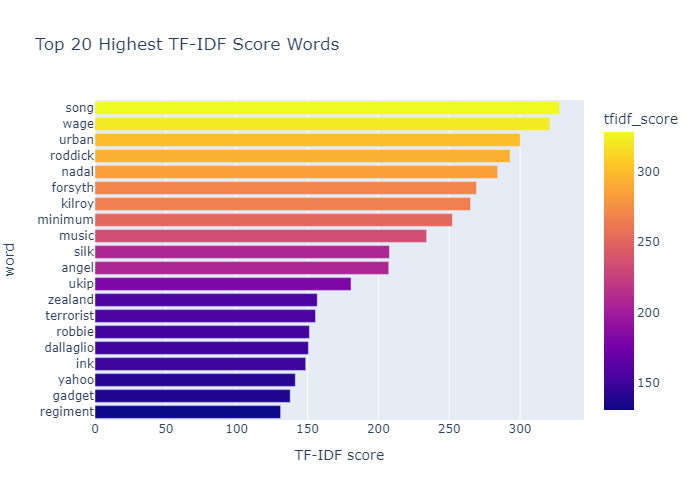
\includegraphics[scale=0.55]{plots/tfidf.png}
  \caption{The top 20 most important words in the BBC News Archive dataset, based of the TF-IDF formula.}
\end{figure}

A high TF-IDF score implies that the word is relevant to the article and important in categorizing it; the opposite is true if the score is low \parencite{manning_raghavan_schütze_2009_tf}. Based on the plot above, it can be inferred that words such as \texttt{"song"} and \texttt{"music"} will useful in properly categorizing entertainment articles, while \texttt{"link"} and \texttt{"gadget"} will be effective in categorizing tech-related articles. Similarly, words like \texttt{"urban"} and \texttt{"terrorist"} can be used to correctly classify political articles. There are 3 obvious categories with topical words that have high TF-IDF scores, however, the 2 remaining categories may present a challenge for a classifier to differentiate from the other categories. TF-IDF can serve as a feature selection technique, allowing the user to control the number of terms in the dataset. This can be achieved by either specifying a maximum number of terms $n$, which selects the top n terms with the highest TF-IDF scores, or by setting a threshold $m$ for the minimum number of times a term must appear in a document to be considered a feature \parencite{manning_raghavan_schütze_2009_tf}. The TF-IDF matrix was used as the baseline, to serve as a point of comparison against the other datasets where DRT was implemented.


%----------------------------------------------------------------------------------------
%	LITERATURE REVIEW SECTION
%----------------------------------------------------------------------------------------
\section{Literature Review}
\hspace{\parindent} Several journal articles were reviewed with the aim of better understanding the effectiveness of the 3 DRTs being investigated. In the study, "Overview and Comparative Study of Dimensionality Reduction Techniques for High-Dimensional Data" conducted by \citeauthor{ayesha_hanif_talib_2020} (\citeyear{ayesha_hanif_talib_2020}), it was shown that LSA was most effective on high-dimensional (HD) textual data, with the ability to understand the context of a word in relation to the document. However, the study found that the LSA method was both computationally and temporally expensive and had a tendency to overfit the model \parencite{ayesha_hanif_talib_2020}. In their paper, "How Dimensionality Reduction Affects Sentiment Analysis NLP Tasks: An Experimental Study", \citeauthor{10.1007/978-3-031-08337-2_25} (\citeyear{10.1007/978-3-031-08337-2_25}) observed that reducing the dimensionality of an HD textual dataset using LSA resulted in an increase in training time as the number of dimensions increased. However, the untreated dataset with a dimension space of $10^4$ needed less training time, and the model accuracy was better compared to the reduced dataset with a dimensionality of $10^3$ \parencite{10.1007/978-3-031-08337-2_25}. A moderate reduction in dimensionality was more time-efficient and had a small to moderate impact on model accuracy \parencite{10.1007/978-3-031-08337-2_25}.

In their paper "Linear Discriminant Analysis in Document Classification", \citeauthor{torkkola2001linear} (\citeyear{torkkola2001linear}) found that using LDA treated data was more effective at minimizing the misclassification error rate than the original untreated dataset. The original dataset, with 5,718 dimensions, resulted in an error rate of 11.2\%, while the LDA reduced dataset, with 513 dimensions, had an error rate of 11.4\% \parencite{torkkola2001linear}. However, the LDA-treated dataset, which had a dimension of 64, resulted in an error rate of 7.8\% \parencite{torkkola2001linear}. Similar to the paper mentioned above, other studies have also highlighted the effectiveness of LDA in selecting the most discriminative words from HDDs and noted the added benefit of reduced train and test time. For example, in the paper "Employing Fisher Discriminant Analysis for Arabic Text Classification" by \citeauthor{abuzeina2018employing} (\citeyear{abuzeina2018employing}), it was found that the use of semantic removed LDA transformed features performed similarly to the semantic-rich LSA extracted features when classifying Arabic text.

In their paper "Deep Variational Auto-Encoder for Text Classification", \citeauthor{8780129} (\citeyear{8780129}) found that AE was more efficient than classical DRTs like PCA in dealing with sparse and discrete data, with an accuracy of 96\% as opposed to PCA's accuracy of 89\%. AE was more efficient on smaller datasets as its performance began to drop on larger datasets \parencite{8780129}. According to the 2019 research article titled "Empirical Comparison between Autoencoders and Traditional Dimensionality Reduction Methods" by \citeauthor{8791727}, AE outperformed classical DRTs, such as PCA, at lower dimensions due to its ability to learn the highly nonlinear nature of the data. However, as the data dimensions increased, PCA's projection improved to retain enough information, reducing the accuracy gap between the two methods \parencite{8791727}. \citeauthor{8791727} (\citeyear{8791727}) observed that the computational time needed to train an AE was on average 2-4 times higher than that of PCA. They advised that PCA be used on larger data as its accuracy is comparable to AE \parencite{8791727}.

\subsection{Latent Semantic Analysis (LSA)}
\hspace{\parindent} LSA is a linear DRT which uses linear functions to transform HDD to lower dimensions \parencite{ayesha_hanif_talib_2020}. As an unsupervised technique, LSA does not require labelled data to transform HDD to lower dimensions. LSA utilizes singular value decomposition (SVD), a linear algebra technique, to reduce the dimensions while retaining the similarity structure of the documents or articles \parencite{dumais_2005}. The articles are typically compared using cosine similarity, where articles with high similarity have a value close to 1 and dissimilar articles have a value close to 0 \parencite{dumais_2005}. However, other methods such as Euclidean distance or Jaccard similarity can also be used for comparison purposes \parencite{dumais_2005}. It should be noted that in LSA, if the requested dimension level is larger than the number of samples the LSA will reduce the dimension to the size of the samples available \parencite{dumais_2005}.

In LSA, the number of features (i.e., columns) in the reduced data matrix is typically chosen to be less than or equal to the number of rows (i.e., samples) in the original data matrix. This is because LSA works by decomposing the original document-term matrix into a smaller set of "latent" topics or concepts, which are represented by the columns of the reduced matrix.

The SVD is used to decompose document-term matrix $A_{m,n}$ into 3 matrices: $U_{m,k}, \Sigma_{k,k}, V^{T}_{k,n}$ \parencite{Sumedha_2018}. Both $U$ and $V^{T}$ are orthonormal matrices, meaning their column vectors have a length of 1 and the dot product of any 2 column vectors equal 0 \parencite{Sumedha_2018}. The document matrix $U$ has documents as rows and latent topics as columns, capturing the relationship between the documents and latent topics \parencite{Sumedha_2018}. The term matrix $V^{T}$ has termed as columns and latent topics as rows, capturing the relationship between the terms and the latent topics \parencite{Sumedha_2018}. The ordered diagonal matrix $\Sigma$ provides the importance value for each latent topic in accurately approximating the original document-term matrix, the values ordered by importance \parencite{Sumedha_2018}. The rank of matrix $A$ is denoted by $k$, which represents the number of latent topics or dimensions a dataset can be reduced to \parencite{Sumedha_2018}. Determining the value of $k$ is the user's responsibility, and the aim of LSA is to find the optimal dimension to reduce to such that $k < n$ while minimizing the error between the original $A_{m,n}$ and the new approximation $A_{m,k}$ \parencite{Sumedha_2018}. After dimension reduction, the document-term matrix $A_{m,k}$ has terms or words represented by latent topics, with a topic possibly having multiple associated terms. This transformed dataset is a significant drawback of LSA, as it can be hard to interpret.

SVD is derived as follows \parencite{Sumedha_2018}:
\begin{equation}
  \begin{aligned}
    A_{m,n} & = U \Sigma V^{T} {T}                                        \\
            & \text{$V$ is the eigenvectors of $A^{T} A$:}                \\
    A^{T} A & = V \Sigma^{2} V^{T}                                        \\
            & \text{$U$ is the eigenvectors of $A A^{T}$:}                \\
    A A^{T} & = U \Sigma^{2} U^{T}                                        \\
    \Sigma  & = \sqrt{\Sigma^{2}}                                         \\
    A_{m,k} & \approx A_{m,n}
    \\ & \approx U_{m,k} \Sigma_{k,k} V^{T}_{k,n}\\
            & \approx \sum_{i = 1}^{k}u_i \sigma_i v_i                    \\
            & \text{$A_{m,k}$ is a good approximation of $A_{m,n}$ when:} \\
            & \min \left\lVert A_{m,n} -A_{m,k}\right\rVert
  \end{aligned}
\end{equation}
where,\\
$A_{m,n}$ = document-term matrix;\\
$U$ = document matrix;\\
$\Sigma$ = latent topics importance value; \\
$V^{T}$ = term matrix; \\
$m$ = number of terms;\\
$n$ = number of documents;\\
$k$ = number of latent topics\\


\subsection{Linear Discriminant Analysis (LDA)}
\hspace{\parindent} Like LSA, LDA is a linear DRT that uses linear transformations to reduce the dimensions of an HDD \parencite{ayesha_hanif_talib_2020}. However, unlike LSA, LDA is a supervised method that requires labelled data to accurately find linear boundaries that separate different categories \parencite{ayesha_hanif_talib_2020}. The goal of LDA is to project the HDD onto a lower-dimensional space with well-defined category boundaries in order to avoid overfitting \parencite{raschka_2014}. However, LDA may not perform well on non-Gaussian datasets since it assumes that the data follows a Gaussian distribution and that the covariance matrix is the same for all categories \parencite{raschka_2014}. Based of these assumptions, LDA computes the mean and covariance matrix for each category and seeks linear combinations of the features such that they maximize the equation: $S = \frac{\sigma^{2}_{between}}{\sigma^{2}_{within}}$ concerning the categories \parencite{raschka_2014}. These linear combinations also referred to as the discriminant functions, are used to transform the HDD to a lower dimension while preserving the class boundaries \parencite{raschka_2014}. Finally, the discriminant functions can be used to categorize new data points based on which category has the highest discriminant function values \parencite{raschka_2014}.

The discriminant function is derived as follows \parencite{Chen_g_2020}:
\begin{equation}
  \begin{aligned}
    a_{i}                & = v^{T}x_{i}                                                               \\
    \mu_{j}              & = \frac{1}{n_{j}} \sum_{x_{i} \in C_{j}} a_{i}                             \\
                         & =  \frac{1}{n_{j}} \sum_{x_{i} \in C_{j}} v^{T}x_{i}                       \\
    \mu_{j}              & = v^{T} m_{j}                                                              \\
    \mu                  & = \frac{1}{n} \sum^{c}_{j = 1} n_{j} \mu_{j}                               \\
                         & = v^{T} \frac{1}{n} \sum^{c}_{j = 1} n_{j} m_{j}                           \\
    \mu                  & = v^{T} m                                                                  \\
    \sigma^{2}_{between} & = \sum^{c}_{j = 1} n_{j} \left( \mu_{j}-\mu \right)^2                      \\
    \sigma^{2}_{between} & = v^{T} S_{B} v                                                            \\
    \sigma^{2}_{within}  & = \sum^{c}_{j = 1} \sum_{x_{i} \in C_{j}} \left( a_{i} - \mu_{j} \right)^2 \\
                         & = v^{T} \sum^{c}_{j = 1} S_{j} v                                           \\
    \sigma^{2}_{within}  & = v^{T} S_{W} v                                                            \\
                         & \therefore \max_{v = k} \frac{\sigma^{2}_{between}}{\sigma^{2}_{within}}   \\
  \end{aligned}
\end{equation}
where,\\
$a_i$ = discriminant function;\\
$v$ = matrix with column vectors k; \\
$x_i$ = a given data point; \\
$k$ = number of vector columns in v;\\
$n_j$ = number of data points from a given category j;\\
$n$ = total number of data points;\\
$c$ = total number of categories;\\
$C_j$ = a given category j; \\
$\mu_{j}$ = mean of a given category;\\
$\mu$ = global mean; \\
$\sigma^{2}_{between}$ = distance category means are from the global mean; \\
$\sigma^{2}_{with}$ = spread within each category; \\


The number of categories in the HDD determines the value of $k$ in LDA \parencite{hastie_friedman_tisbshirani_2017}. In the context of this paper, applying LDA to the dataset would result in reducing the original dimensionality from 24,134 to 4; $ k=c-1$. Each dimension (or category) is associated with a set of terms that are most closely related to that topic \parencite{hastie_friedman_tisbshirani_2017}.

\subsection{Auto-Encoder (AE)}
\hspace{\parindent} The AE is an unsupervised neural network that can encode datasets effectively, thereby reducing their dimensions \parencite{8780129}. It is comprised of three primary layers: an input layer, where the input data is received, a hidden layer, which compresses the dimensions of the original data to a specific dimension (i.e., encoding), and an output layer, where the original dataset is reconstructed from the encoding layer (i.e., decoding) \parencite{8780129}. Unlike the other DRTs mentioned above, AE is able to learn non-linear relationship present in the data \parencite{8780129}. Both the encoder and decoder layers are activated by an activation function that determines which nodes in the layers should be on or off, based on the input layer \parencite{hastie_friedman_tisbshirani_2017_nn}. Through the use of backpropagation AE learns to accurately map the input data to the output data, adjusting the weights and biases in the network to improve the mapping accuracy \parencite{hastie_friedman_tisbshirani_2017_nn}. Backpropagation computes the error between the predicted and actual output and uses this error to retrain and adjust the weights and biases in order to minimize the error \parencite{hastie_friedman_tisbshirani_2017_nn}. The neural network can learn complex relationships from data through this technique, however, it may consume a significant amount of computational resources and time \parencite{hastie_friedman_tisbshirani_2017_nn}.

\begin{center}
  \resizebox{.60\textwidth}{!}{%
    \begin{neuralnetwork}[height=5]
      \newcommand{\nodetextclear}[2]{}
      \newcommand{\nodetextx}[2]{$x_#2$}
      \newcommand{\nodetexty}[2]{$y_#2$}
      \inputlayer[count=4, bias=false, title=Input\\layer, text=\nodetextx]
      \hiddenlayer[count=2, bias=false, title=Hidden\\layer, text=\nodetextclear] \linklayers
      \outputlayer[count=4, title=Output\\layer, text=\nodetextx] \linklayers
    \end{neuralnetwork}}
\end{center}

The above diagram is of a typical auto-encoder architecture consisting of two parts: an encoder (input layer and hidden layer) and a decoder (hidden layer and output layer) \parencite{8780129}. The encoder and decoder are derived as follows \parencite{Sigal_2017}; \parencite{stewart_2023}:
\begin{equation}
  \begin{aligned}
    e,d           & = \min_{e,d}  \left\lVert x-(e\circ d)x \right\rVert^2                           \\
    e             & = \sigma(Wx + b)                                                                 \\
    d             & = \hat{\sigma}(\hat{W}e + \hat{b})                                               \\
    \hat{W}       & = W^{T}                                                                          \\
    l (x,\hat{x}) & = \left\lVert x-\hat{x} \right\rVert ^2                                          \\
                  & = \left\lVert x - \hat{\sigma}(\hat{W}(\sigma(Wx + b))+ \hat{b}) \right\rVert ^2 \\
    \mathcal{L}   & = (1/N) * sum(l(x_i, \hat{x}_i))                                                 \\
                  & \min \mathcal{L}                                                                 \\
  \end{aligned}
\end{equation}
where,\\
$e$ = encoder network; \\
$d$ = decoder network;\\
$W$ = weight matrix;\\
$\sigma$ = an activation function; \\
$\hat{\sigma}$ = an activation function; \\
$x$ = input data;\\
$\hat{x}$ = approximation of the input data;\\
$l$ = loss function; \\
$b$ = b is the bias vector;\\
$\mathcal{L}$ = total number of data points;\\

The weight matrix $W$ captures the relevant patterns and relationships in the input data, according to \citeauthor{hastie_friedman_tisbshirani_2017_nn} (\citeyear{hastie_friedman_tisbshirani_2017_nn}). The number of rows in the matrix corresponds to the number of dimensions in the decoded output data, while the number of columns corresponds to the number of dimensions in the original input data \parencite{hastie_friedman_tisbshirani_2017_nn}. The bias vector allows each neuron to make predictions by adjusting the activation function left or right \parencite{hastie_friedman_tisbshirani_2017_nn}. AE utilizes backpropagation to iteratively minimize the average loss function $\mathcal{L}$ across the entire training set \parencite{hastie_friedman_tisbshirani_2017_nn}.
%----------------------------------------------------------------------------------------
%	EXPERIMENT SECTION
%----------------------------------------------------------------------------------------
\section{Experiment}
\hspace{\parindent} Four metrics were used to compare the 3 DRTs: cosine similarity, which measures the degree to which the DRTs preserve the semantic structure of the original data; reconstruction error, which quantifies the difference between the original data and the reduced data via the mean squared error; classification accuracy, which evaluates the accuracy of a classifier trained on the reduced dataset generated by each DRT; and computational time, which assesses how long it takes for each DRT to generate the reduced dataset.

\subsection{Design}
\hspace{\parindent} Two commonly used text classifiers, Random Forest (RF) and Support Vector Machine (SVM), were employed during this experiment. As the focus of the paper was on DRTs, the classifiers' hyperparameters were not fine-tuned; they were left at their default settings as determined by the \texttt{sklearn} library. An important advantage of doing this was that the same classifier would be used for all the reduced datasets. To ensure reproducibility of the experiment, a random seed was set. A randomized stratified training and test set were used for each DRT trial run, with a 70/30 data split. As the categories were fairly balanced, stratified sampling was selected to ensure that the training and testing datasets reflect this balance. Baseline results were obtained using the untreated TF-IDF matrix. The DRTs were used to reduce the dimensions of the original data by 2\%, 1\%, and 0.1\%, except for LDA which does not allow users to set the level of dimension reduction. To account for this, an additional reduction dataset was created for each of the other DRTs with the same dimensions as the LDA reduced dataset. For consistency, the untreated TF-IDF was also partitioned in the same way as the reduced dataset generated by DRTs. The classifiers were then applied to these resulting datasets, and the four metrics mentioned earlier were used to evaluate the performance of the DRTs. The experiment was conducted on a PC with the following specifications: Intel(R) Core(TM) i7-7700 CPU at 3.60GHz processor, 16 GB of RAM, and Windows 10 Pro operating system. All experimental and EDA work was completed using \texttt{python} version 3.7.10 \parencite{10.5555/1593511}.

\subsection{Results}
\hspace{\parindent} TF-IDF, LSA, and LDA dimension reduction were performed using the \texttt{sklearn} library in \texttt{python}, while AE dimension reduction was implemented using the \texttt{keras} library \parencite{pedregosa2011scikit}; \parencite{chollet2015keras}. The activation function for the AE was selected following best practices outlined by \citeauthor{goodfellow_bengio_courville_2017} (\citeyear{goodfellow_bengio_courville_2017}) in their book "Deep Learning." Specifically, the relu activation function was used for the encoder and sigmoid for the decoder. The batch size of 64 and epoch of 10 was selected based on the recommendations in the same book \parencite{goodfellow_bengio_courville_2017}.

\subsubsection{Computational Time}
\begin{figure}[H]
  \centering
  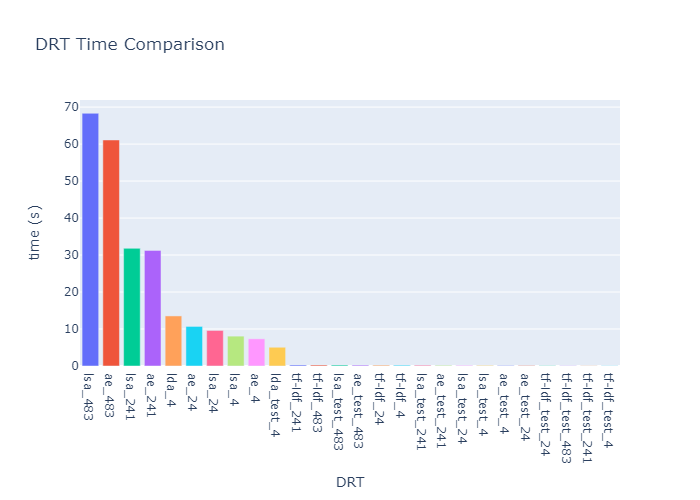
\includegraphics[scale=0.60]{plots/time.png}
  \caption{The computational time it took for each DRT to transform the train and test datasets.}
\end{figure}

\hspace{\parindent} The TF-IDF DRT method was very efficient, taking less than 1 second, approximately 0.1 second, to compute regardless of the dimension reduction size. In contrast, both AE and LSA were far more computationally demanding, with AE being more computationally expensive than LSA. The AE method took over 50 seconds to train and compress the original data by 2\%, but once trained, it was the second fastest DRT to transform the test data after TF-IDF. On the other hand, LSA, on average, took the longest time to transform the train and test data, regardless of the dimension reduction level. Based solely on computation time, LDA was the most efficient DRT method, taking only 13 seconds to transform the train set and 5 seconds to transform the test set.

\subsubsection{Cosine Similarity and Reconstruction Error}
\begin{figure}[H]
  \centering
  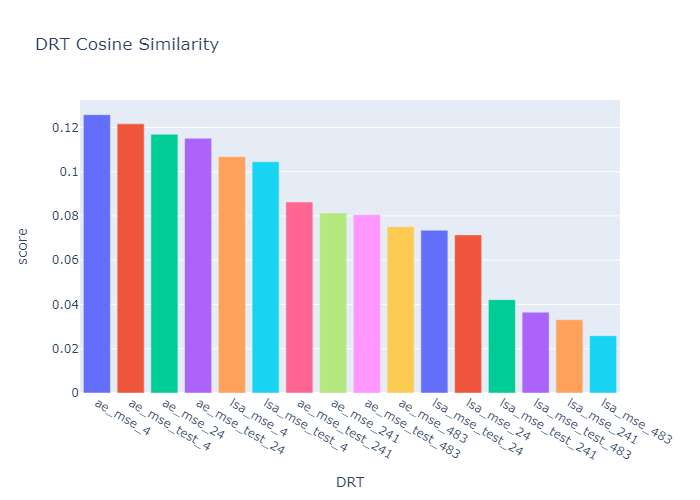
\includegraphics[scale=0.60]{plots/cs.png}
  \caption{The cosine similarity between the train and test sets each for DRT.}
\end{figure}

\hspace{\parindent} Out of the 3 DRTs that were tested, the AE had the highest cosine similarity value when comparing the reduced training and test sets. The larger the dimension of the reduced datasets, the higher the cosine similarity. However, given the low magnitude of the cosine similarity values, it can be inferred that the reduced datasets have very little in common with the original data, which might affect their effectiveness during the classification task.

\begin{figure}[H]
  \centering
  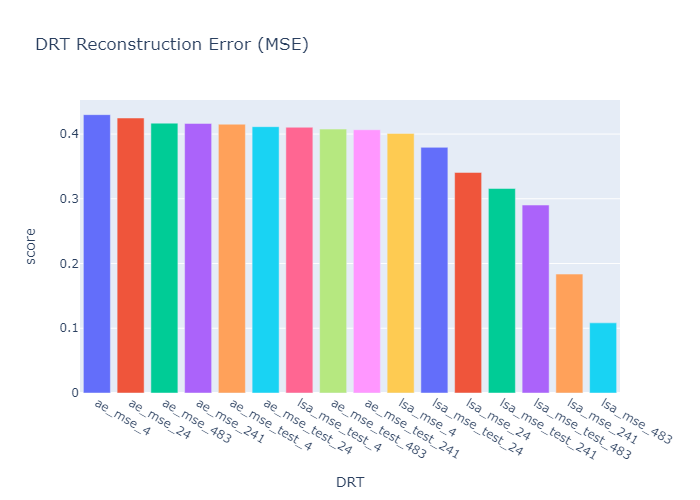
\includegraphics[scale=0.60]{plots/re.png}
  \caption{The reconstruction error for the train and test sets each for DRT.}
\end{figure}

LSA had the smallest and largest reconstruction error scores, depending on the dimension size and dataset used, while the AE's scores were consistent regardless of the dimension size. As the dimension size of LSA reduced, the training set error rate also decreased, but as the dimension size of LSA reduced, the test set error rate increased. This could be because reconstructing higher-dimensional data involves more relationships among the data points, resulting in more room for error. However, with fewer points present in the test data, there might be fewer informative relationships, and an increase in dimensions allows more informative relationships to be mapped. LDA along with TF-IDF could not have their reconstruction error calculated due to the way they transform the data.

\subsubsection{Classification accuracy}

\begin{figure}[H]
  \centering
  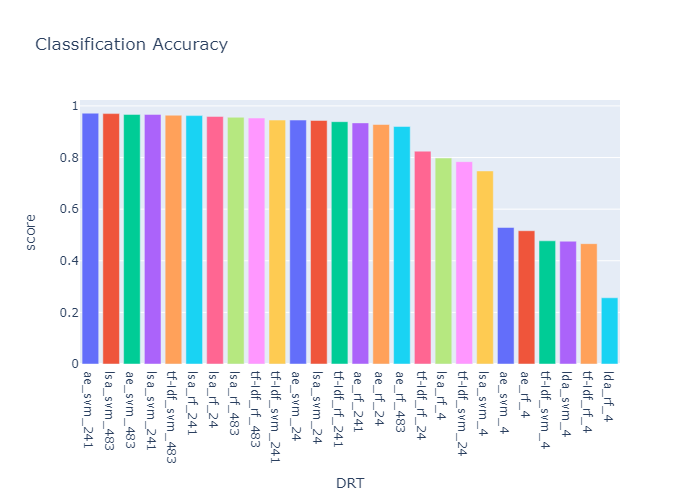
\includegraphics[scale=0.60]{plots/ca.png}
  \caption{The classification accuracy on SVM and RF for each for DRT.}
\end{figure}

\hspace{\parindent} The feature selection method, TF-IDF, was the best reduction method based on classification accuracy. Nearly all the TF-IDF reduced data produced an accuracy above 75\%, except for the 4-dimensional reduced dataset. The results of the TF-IDF were expected, as classification accuracy generally improves as dimensions increase. However, the drop in accuracy of those TF-IDF reduced datasets from 24 dimensions to 4 dimensions was significant. The next best DRT was LDA, with the 4-dimensional reduced dataset paired with an SVM classifier producing almost 50\% accuracy. All the LSA-treated data produced an overall accuracy range of 30\% to 40\%, while AE-treated data yielded an overall accuracy range of 20\% to 40\%. The performance of all the DRTs tested, except for TF-IDF, was poor, likely due to the small size of the reduced datasets.
%----------------------------------------------------------------------------------------
%	CONCLUSION SECTION
%----------------------------------------------------------------------------------------
\section{Conclusion}
\hspace{\parindent} To summarize, the TF-IDF method proved to be the most efficient and effective reduction technique in terms of classification accuracy and computational time. The study explored three DRTs - LSA, LDA, and AE - and found that LSA was the best at compressing information, but its stability was a concern, while AE was the most stable DRT, producing consistent results in both classification accuracy and reconstruction error. Given the increasing advancements in NLP, these 3 DRTs showcase classical ways of handling overfitting during a text classification task. Although the above results may appear poor, it is worth noting that given the significant reduction in dimension, the DRTs worked fairly well in capturing enough information from the original dataset to yield an accuracy range of 20-50\%. The range of the reduction explored was based solely on the limitation of the PC used. The DRTs cannot replace proper data processing for the task at hand, but they can be useful in reducing noise and computation time, as demonstrated by the performance of TF-IDF treated models.

Future research could investigate the optimal dimension levels for each DRT using GPUs or cloud services and explore the relationship between DRT and reconstruction error. In general, there are several intersections between NLP and DRT that warrant further investigation.


\newpage
bob\\
The encoder and decoder are derived as follows \parencite{Sigal_2017}; \parencite{stewart_2023}:
\begin{equation}
  \begin{aligned}
    e,d           & = \min_{e,d}  \left\lVert x-(e\circ d)x \right\rVert^2                           \\
    e             & = \sigma(Wx + b)                                                                 \\
    d             & = \hat{\sigma}(\hat{W}e + \hat{b})                                               \\
    \hat{W}       & = W^{T}                                                                          \\
    l (x,\hat{x}) & = \left\lVert x-\hat{x} \right\rVert ^2                                          \\
                  & = \left\lVert x - \hat{\sigma}(\hat{W}(\sigma(Wx + b))+ \hat{b}) \right\rVert ^2 \\
    \mathcal{L}   & = (1/N) * sum(l(x_i, \hat{x}_i))                                                 \\
                  & \min \mathcal{L}                                                                 \\
  \end{aligned}
\end{equation}
where,\\
$e$ = encoder network; \\
$d$ = decoder network;\\
$W$ = weight matrix;\\
$\sigma$ = an activation function; \\
$\hat{\sigma}$ = an activation function; \\
$x$ = input data;\\
$\hat{x}$ = approximation of the input data;\\
$l$ = loss function; \\
$b$ = b is the bias vector;\\
$\mathcal{L}$ = total number of data points;\\
\newpage
\printbibliography
\end{document}
